\section{Aufbau}
\label{sec:Aufbau}
\begin{figure}
    \centering
    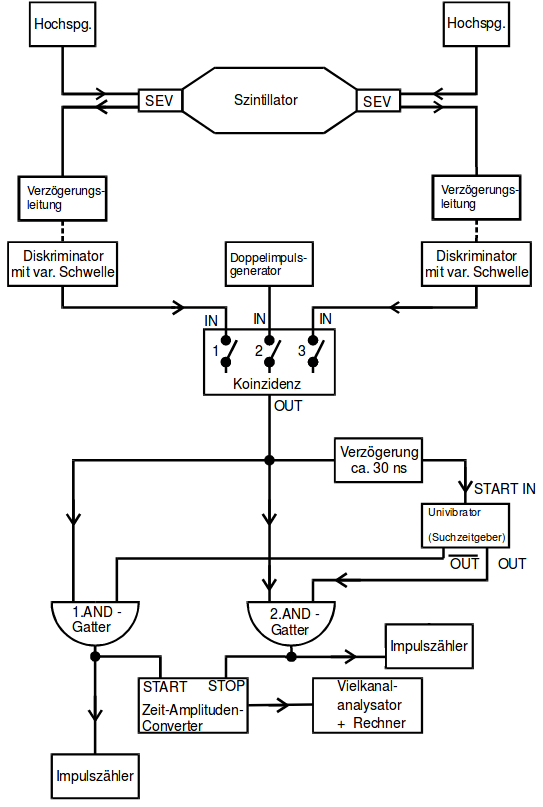
\includegraphics[width=0.9\textwidth]{content/images/AufbauV01.png}
    \caption{Die Messschaltung zur Aufnahme von Individuallebensdauern kosmischer Myonen,nach \cite{V01}.}
    \label{fig:Aufbau}
    \end{figure}
%Bild muss noch angepasst werden(zweite verzögerungsleitung, zweiter impulszähler)
%Der Aufbau besteht aus zwei Teilen. Der erste Teil filtert möglichst alle Impulse heraus, die aufgrund von. Im Anschluss folgt eine Schaltung, welche die individuellen Zerfallszeiten misst und sie in eine für den Computer verwertbare Form umformt.
%gehört die funktion vom szintillator hierrein
 Die in der Atmosphäre entstandenen Myonen gelangen zunächst in einen Szintillator. Es wird zwischen organischen und anorganischen Szintillatoren unterschieden. Die organischen Szintillatoren besitzen eine gute Zeitauflösung, dafür jedoch eine geringere Energieauflösung. Bei den anorganischen Szintillatoren ist es umgekehrt. Da der Versuch eine hohe Zeitauflösung benötigt, während die Energie der Myonen nicht betrachtet wird, wird ein organischer Szintillator gewählt. In diesem werden die zunächst noch relativistischen Myonen abgebremst, wobei sie ihre kinetische Energie an die umliegenden Moleküle abgeben. Diese werden daraufhin in energetisch höhere Niveaus gehoben und kehren daraufhin unter Aussendung eines Photons wieder in ihren Grundzustand zurück. Die Photonen befinden sich energetisch am oberen Rand des sichtbaren Spektrums. Im Anschluss werden die Photonen mithilfe zweier Photomultiplier in elektrische Impulse umgewandelt und verstärkt.
 %"befinden sich" besser als "liegen"?
  %Anschließend werden die Lichtquanten in zwei an beiden Seiten des Szintillators befestigten Photomultipliern in elektrische Signale umgewandelt und zur Verwertbarkeit um ca. um den Faktor $10^6$ verstärkt.
   Danach passieren die Impulse auf beiden Seiten eine Verzögerungsleitung und einen Diskriminator. Mithilfe der Koinzidenz können Fehlstellen in den Leitungen ausgeglichen werden, sodass die im Szintillator auftretenden Impulse gleichzeitig in die Koinzidenz gelangen. In den Diskriminatoren werden die Signale einerseits von Störimpulsen niederer Spannung gefiltert und andererseits in logische Signale umgeformt, welche von der nachfolgenden Koinzidenzapperatur benötigt wird.
    %Die zweite Stufe der Filterung von Störquellen bildet eine Koinzidenzapperatur.
     Diese gibt ein Signal aus, falls gleichzeitig Impulse an beiden Eingängen auftreten. Ursache des Untergrunds sind jedoch hauptsächlich thermische Elektronen, welche in den Photomultipliern entstehen und in diesen anschließend soweit verstärkt werden, sodass sie den Schwellwert der Diskriminatoren überschreiten. Da das Auftreten thermische Elektronen jedoch zufällig geschieht, ist es nur sehr unwahrscheinlich, dass 2 Impulse im benötigten
    %"stochastisch" besser als "zufällig"
     Abstand auftreten. Die Photonen bewegen sich hingegen schnell genug, sodass die durch Myonen hervorgerufenen Impulse die Koinzidenzapperatur passieren können.
    %unterer teil der schaltung
   Nachdem der Untergrund nun hinreichend herausgefiltert worden ist, lässt sich nun die Lebensdauer der Myonen bestimmen. Ausschlaggebend hierfür sind Myonen, welche bereits in der Atmosphäre ausreichend abgebremst worden sind und im Szintillator nun zum Stillstand kommen, wo sie gemäß Gleichung $\eqref{eq:zerfall}$ zerfallen.
    % Da die vorherige Zeitdilatation nun aufhört zu wirken, kommt es zum Zerfall der Myonen.
    % sollte das mit den myonen vll doch eher in die theorie ?
    Die entstehenden Produkte besitzen eine hohe kinetische Energie und werden ihrerseits im Szintillator abgebremst, wodurch ein zweiter Impuls ausgesendet wird. Die Zeitdifferenz beider Impulse liefert die individuelle Lebensdauer des Myons. Die Messschaltung nach Abb.$ \ref{fig:Aufbau}$ funktioniert folgendermaßen:

    Anfangs liegt an allen Komponenten bis zu den AND-Gattern kein Impuls an. Daher sind bis auf den $\overline{\text{OUT}}$ Ausgang des Univibrators alle Ein und Ausgänge auf 0 geschaltet.
    Liegt nun der erste Impuls an beiden AND-Gattern an, so wird er, da der Univibrator auf 0 und der $\overline{\text{OUT}}$ Ausgang daher auf 1 steht, nur an dem AND-Gatter 1 hindurchgelassen. Dort startet er die Zeitmessung im TAC und wird zusätzlich mithilfe eines Impulszählers registriert. Nach ca. $SI{30}{\nano\second}$ passiert der Impuls die Verzögerungsleitung und liegt am Univibrator an. Die Verzögerungszeit ist so gewählt, dass der Impuls das 1. AND-Gatter bereits passiert hat, bevor das Signal am Univibrator anliegt. Dieser klappt sich nun für die Dauer der eingestellten Suchzeit $T_\text{S}$ auf 1 um, weswegen sich der $\overline{\text{OUT}}$ auf 0 und der OUT auf 1 umklappt. Liegt nun ein zweiter Impuls an den Komponenten an, so gelangt dieser nur durch das 2 AND Gatter, wird dort über einen zweiten Impulszähler registriert und stoppt die Messung im TAC. Letzterer gibt daraufhin eine proportional zur Zeit erhöhte Spannung an einen angeschlossenen Vielkanalanalysator mit 512 Kanälen weiter. In diesem werden die Impulse ihrer Höhe nach in einzelne Kanäle einsortiert und in jedem einzelnen wird die Anzahl der eintreffenden Impulse gezählt. Die Messdaten können mit einem angeschlossenen Computer ausgelesen werden. Gelangt in der Zeit $T_\text{S}$ kein weiterer Impuls in die Schaltung, klappt der Univibrator wieder zurück und der nächste Impuls wird als neues Startsignal gewertet. Kommt es in der Zeit $T_\text{S}$ zur Abbremsung von zwei verschiedenen Myonen so werden diese als ein Zerfall gewertet. Dieser Untergrund lässt sich nicht herausfiltern und muss nachträglich bestimmt werden. Damit möglichst viele Zerfälle erfasst werden können, muss die Suchzeit deutlich größer als die erwartete charakteristische Lebensdauer gewählt werden. Andererseits muss sie für eine erfolgreiche Trennung zweier aufeinanderfolgender Zerfälle auch deutlich kleiner sein als die erwartete Zeit zwischen zwei Zerfällen. Daher wird eine Suchzeit von $\SI{\micro}{\second}$ gewählt. 
%dieses problem mit dem resetten nach dem 2. impuls fehlt noch


    %Der erste Impuls läuft zu beiden AND-Gattern. Da das 1. AND-Gatter über den $\overline{\text{OUT}}$  und das 2. AND-Gatter über den OUT-Zugang eines Univibrators verbunden ist, wird der Impuls nur am 1. AND-Gatter durchgelassen. Er gelangt anschließend in den angeschlossenen Startimpulszähler und in den TAC, wo er die Zeitmessung startet. Mit ca. $\SI{30}{\nano\second}$ Verzögerung gelangt der Impuls auch in den Univibrator. Dieser klappt nun für eine eingestellte Zeit $T_\text{S}$ um. Gelangt in dieser Zeit ein zweiter Impuls in die Schaltung, wird dieser durch das 2. AND-Gatter in den TAC und einen zweiten Impulszähler für die Stops weitergeleitet. Der TAC stoppt daraufhin die Messung und gibt einen proportional zur Zeit angestiegenen Strom an einen angeschlossenen Vielkanalanalysator mit 512 Kanälen weiter. In diesem werden die Impulse ihrer Höhe nach in einzelne Kanäle einsortiert und in jedem einzelnen wird die Anzahl der eintreffenden Impulse gezählt. Die Messdaten können mit einem angeschlossenen Computer ausgelesen werden. Gelangt in der Zeit $T_\text{S}$ kein weiterer Impuls in die Schaltung, klappt der Univibrator wieder zurück und der nächste Impuls wird als neues Startsignal gewertet. Kommt es in der Zeit $T_\text{S}$ zur Abbremsung von zwei verschiedenen Myonen so werden diese als ein Zerfall gewertet. Dieser Untergrund lässt sich nicht herausfiltern und muss nachträglich bestimmt werden.